\documentclass[11pt, a4paper]{article}

% --- PAQUETES DE CONFIGURACIÓN BÁSICA ---
\usepackage[utf8]{inputenc}
\usepackage[T1]{fontenc}
\usepackage[spanish, es-nodecimaldot]{babel}
\usepackage{graphicx}
\usepackage[top=2.2cm, bottom=2.5cm, left=2.2cm, right=2.2cm]{geometry}
\usepackage{caption}
\usepackage{float}
\usepackage{microtype}
\usepackage{xcolor}
\usepackage[colorlinks=true, linkcolor=blue!70!black, urlcolor=blue!70!black, citecolor=blue!70!black]{hyperref}

% Configuración de títulos y figuras
\captionsetup{font=small, labelfont=bf, justification=centering}

\title{\textbf{Trabajo Práctico 3: Big Push y Crecimiento Equilibrado vs. Desequilibrado}\\[0.3em]
\large Evidencia Empírica para la India (1960--2025)}
\author{\textbf{Mateo Barros} \& Grupo de Estudio \\[0.2em]
\textit{Desarrollo Económico -- Licenciatura en Economía} \\
\textit{Universidad Nacional del Sur (UNS)}}
\date{Septiembre de 2026}

\begin{document}

\maketitle

\vspace{-1em}
\noindent\rule{\textwidth}{0.6pt}
\vspace{0.5em}

\section{Parte 1: Big Push e Infraestructura Complementaria}

El marco teórico de \textit{Big Push} (Rosenstein-Rodan; Murphy, Shleifer y Vishny) plantea que el desarrollo requiere de una aceleración sostenida del crecimiento acompañada por un salto coordinado de la inversión y la coevolución simultánea de infraestructura y complementariedades de red (\textit{Social Overhead Capital}).

\subsection{Dinámica Macroeconómica de Crecimiento e Inversión}

La Figura~\ref{fig:macro_hist} presenta la evolución completa de largo plazo (1960--2025) de las tasas de acumulación de capital y la trayectoria del ingreso por habitante.

\begin{figure}[H]
    \centering
    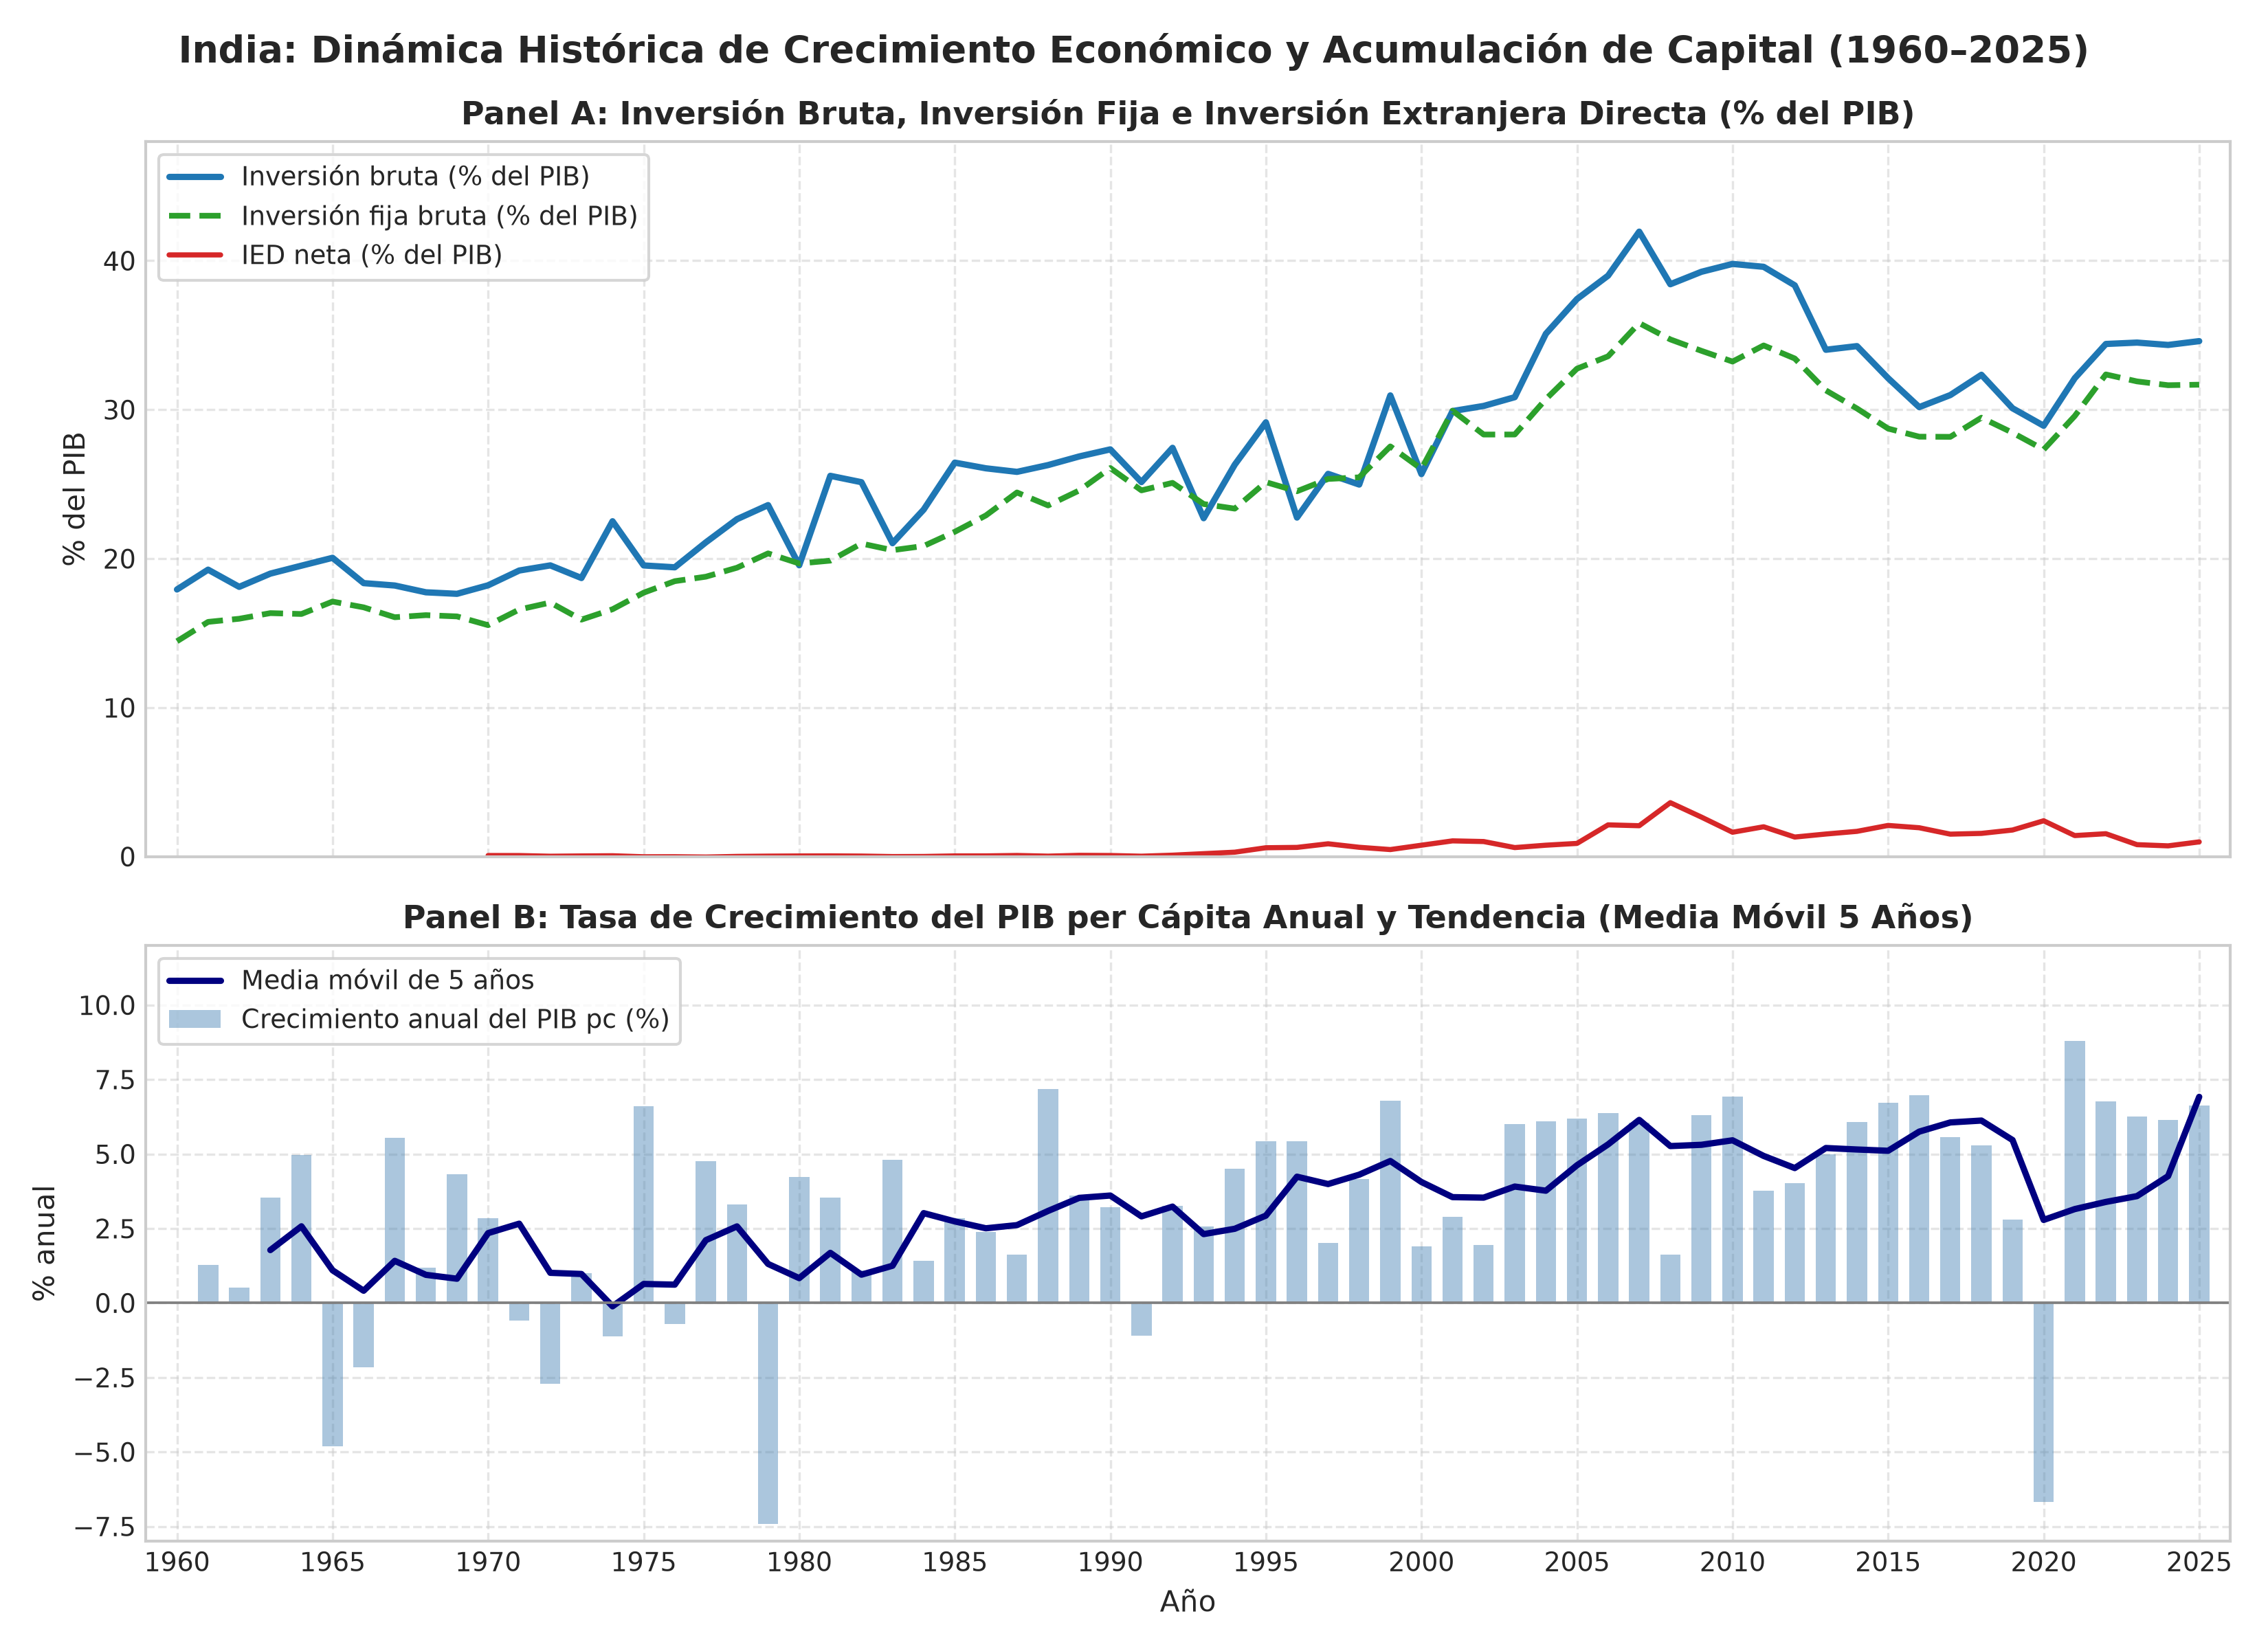
\includegraphics[width=0.98\textwidth]{output/figures/fig1_india_crecimiento_inversion_historico.png}
    \caption{\textbf{India: Crecimiento del PIB per Cápita, Inversión e IED (1960--2025).} \\
    \textit{Panel A:} Inversión bruta, inversión fija bruta e IED neta (\% del PIB). \textit{Panel B:} Crecimiento anual del PIB per cápita y tendencia de largo plazo (media móvil de 5 años). Fuente: World Bank (WDI).}
    \label{fig:macro_hist}
\end{figure}

\noindent \textbf{Descripción breve:} Entre 1960 y 1990 la tasa de inversión fluctuó en niveles moderados (15--22\% del PIB) y la IED fue virtualmente inexistente ($<0.1\%$). A partir de las reformas de 1991 y con fuerza en los años 2000, la inversión bruta experimentó un salto estructural que superó el 40\% del PIB, coincidiendo con una tasa promedio de crecimiento per cápita superior al 6\% anual.

\vspace{1em}
\subsection{Infraestructura de Transporte y Movilidad}

La Figura~\ref{fig:transporte} analiza las series físicas de transporte para evaluar si la logística actuó como cuello de botella o facilitador del proceso productivo.

\begin{figure}[H]
    \centering
    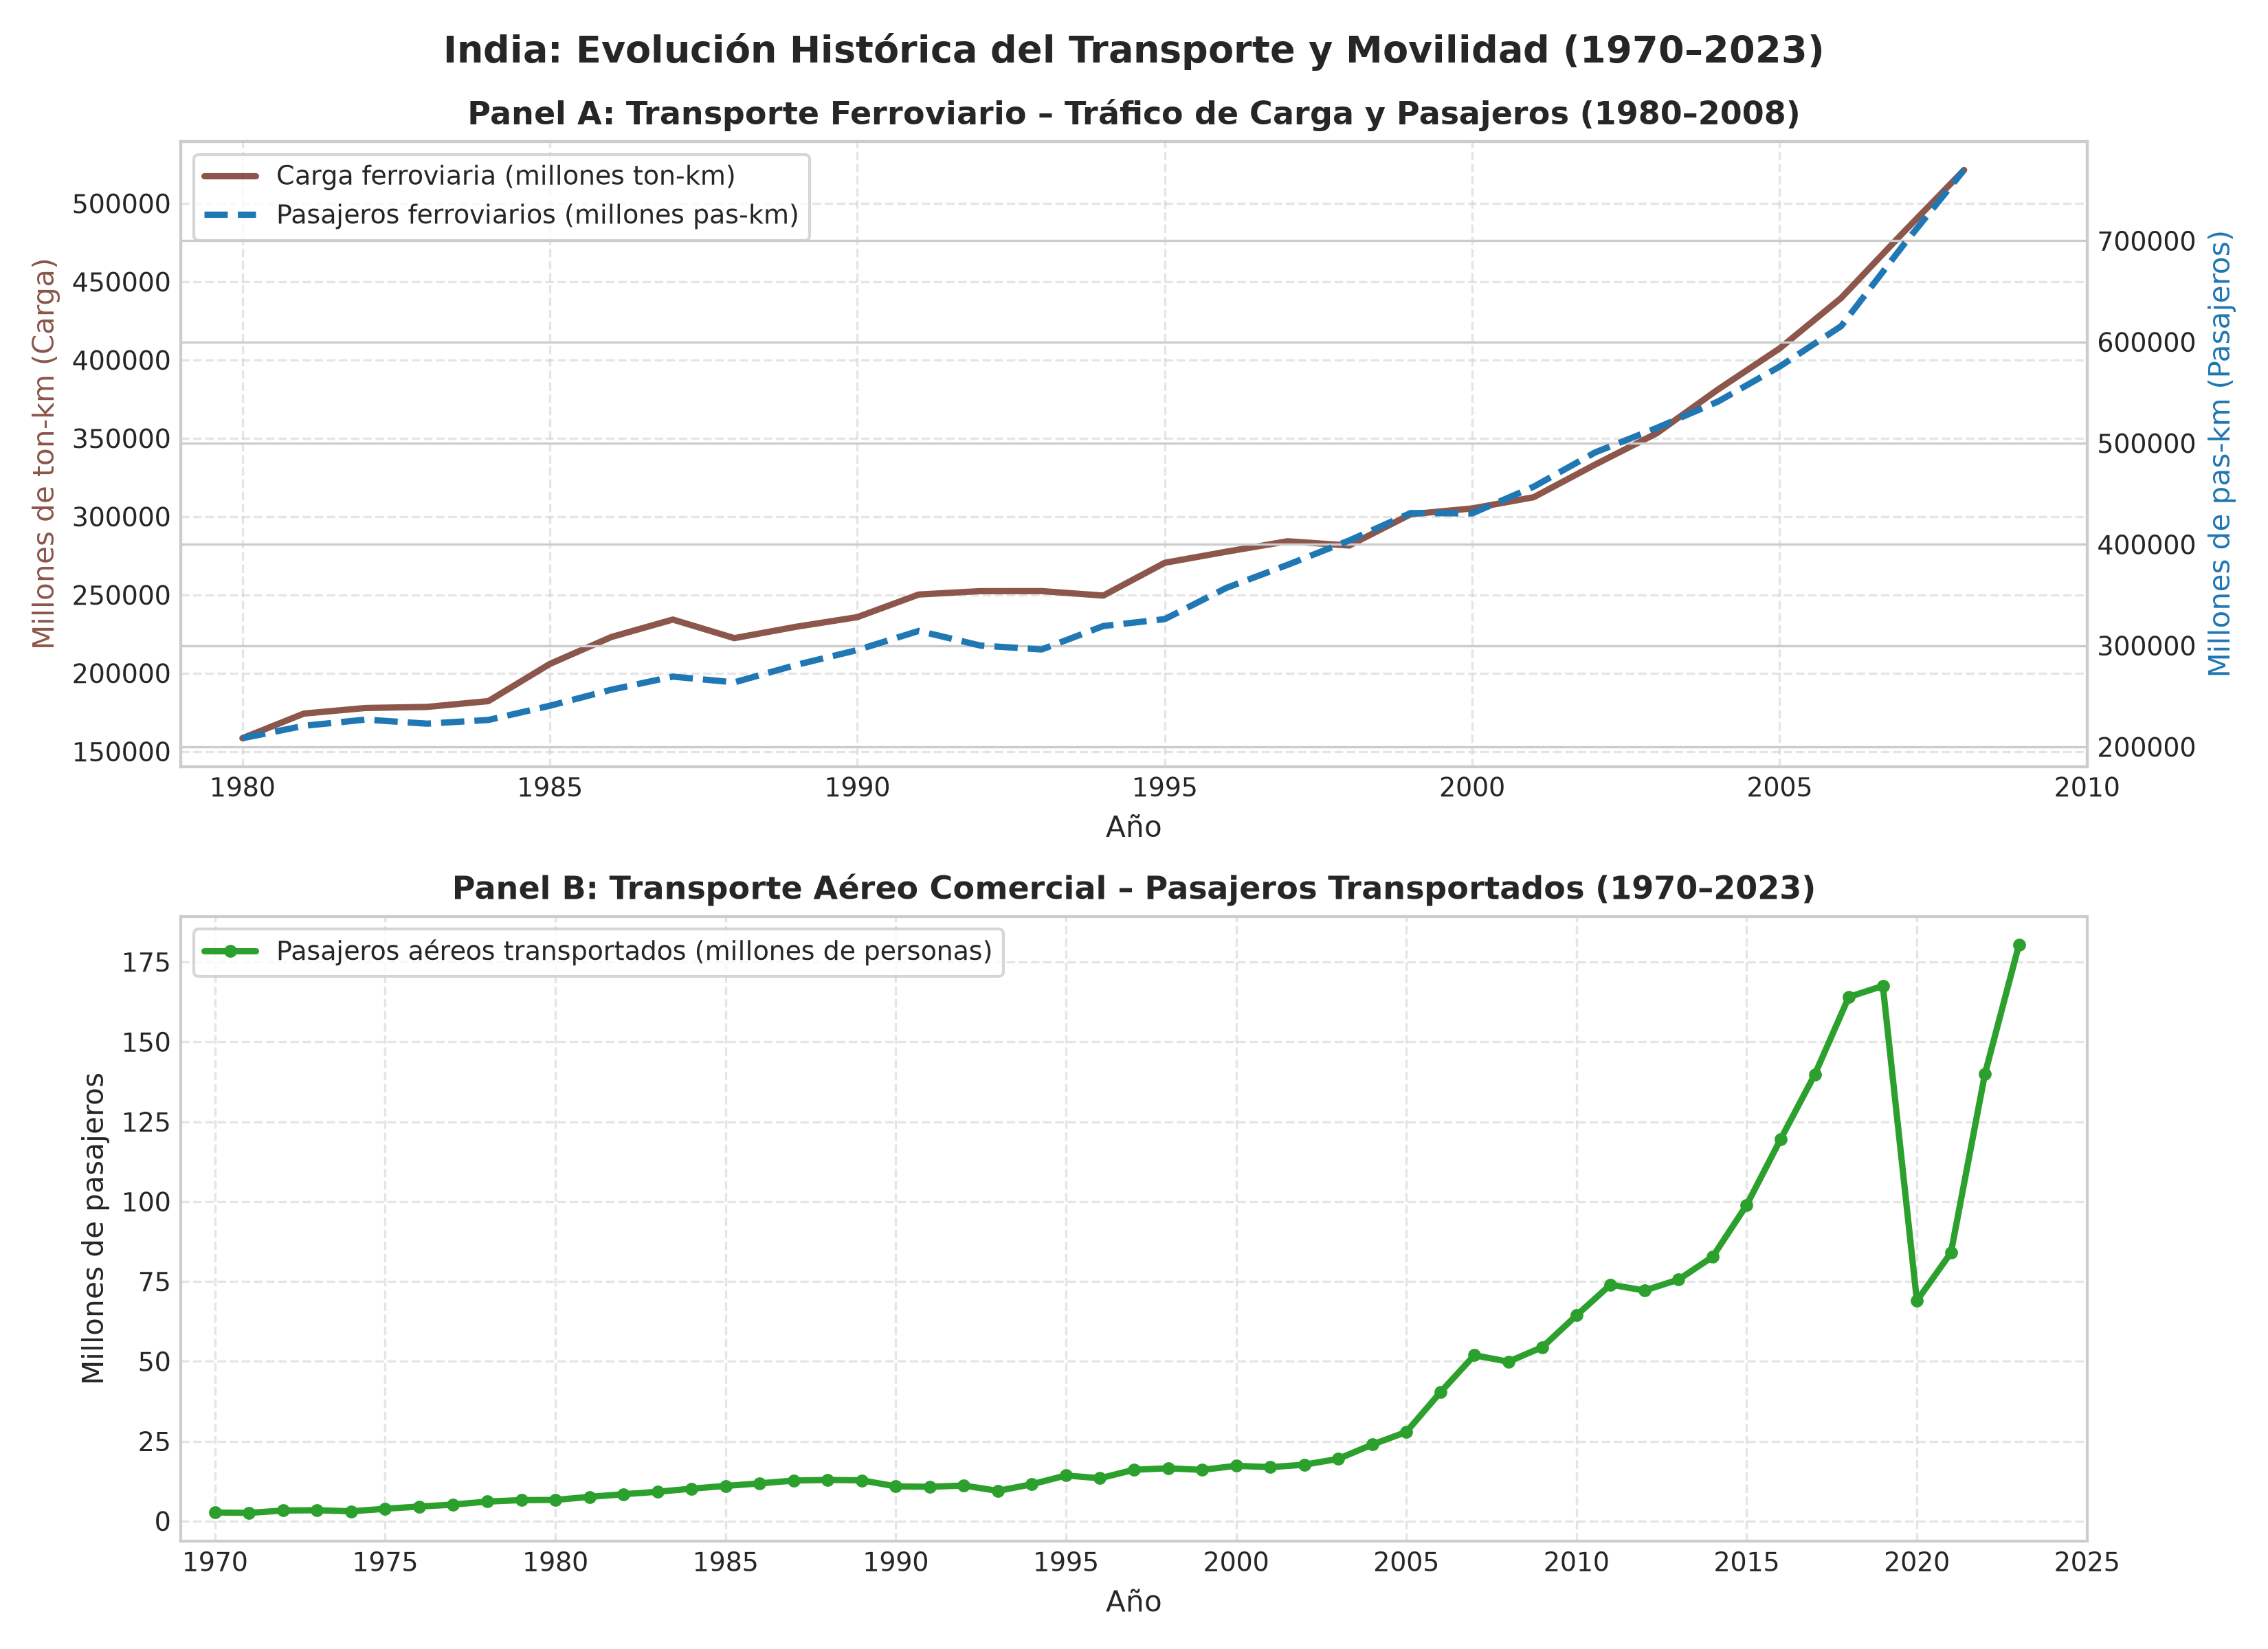
\includegraphics[width=0.98\textwidth]{output/figures/fig2_india_transporte_historico.png}
    \caption{\textbf{India: Evolución Histórica de Infraestructura de Transporte (1970--2023).} \\
    \textit{Panel A:} Tráfico ferroviario de carga (millones ton-km) y pasajeros (millones pas-km), 1980--2008 (EconStats). \textit{Panel B:} Transporte aéreo comercial de pasajeros en millones de personas, 1970--2023 (World Bank).}
    \label{fig:transporte}
\end{figure}

\noindent \textbf{Descripción breve:} La red ferroviaria absorbió el salto productivo de la industria pesada y la minería, multiplicando la carga de 150.000 a más de 520.000 millones de ton-km. Simultáneamente, el transporte aéreo comercial despegó de 13 millones de pasajeros en 2000 a más de 180 millones en 2023, facilitando la integración del pujante sector de servicios y tecnología.

\newpage
\subsection{Infraestructura de Energía y Telecomunicaciones}

La Figura~\ref{fig:energia_telecom} documenta la indivisibilidad del capital básico en potencia eléctrica y la rápida transición tecnológica en conectividad.

\begin{figure}[H]
    \centering
    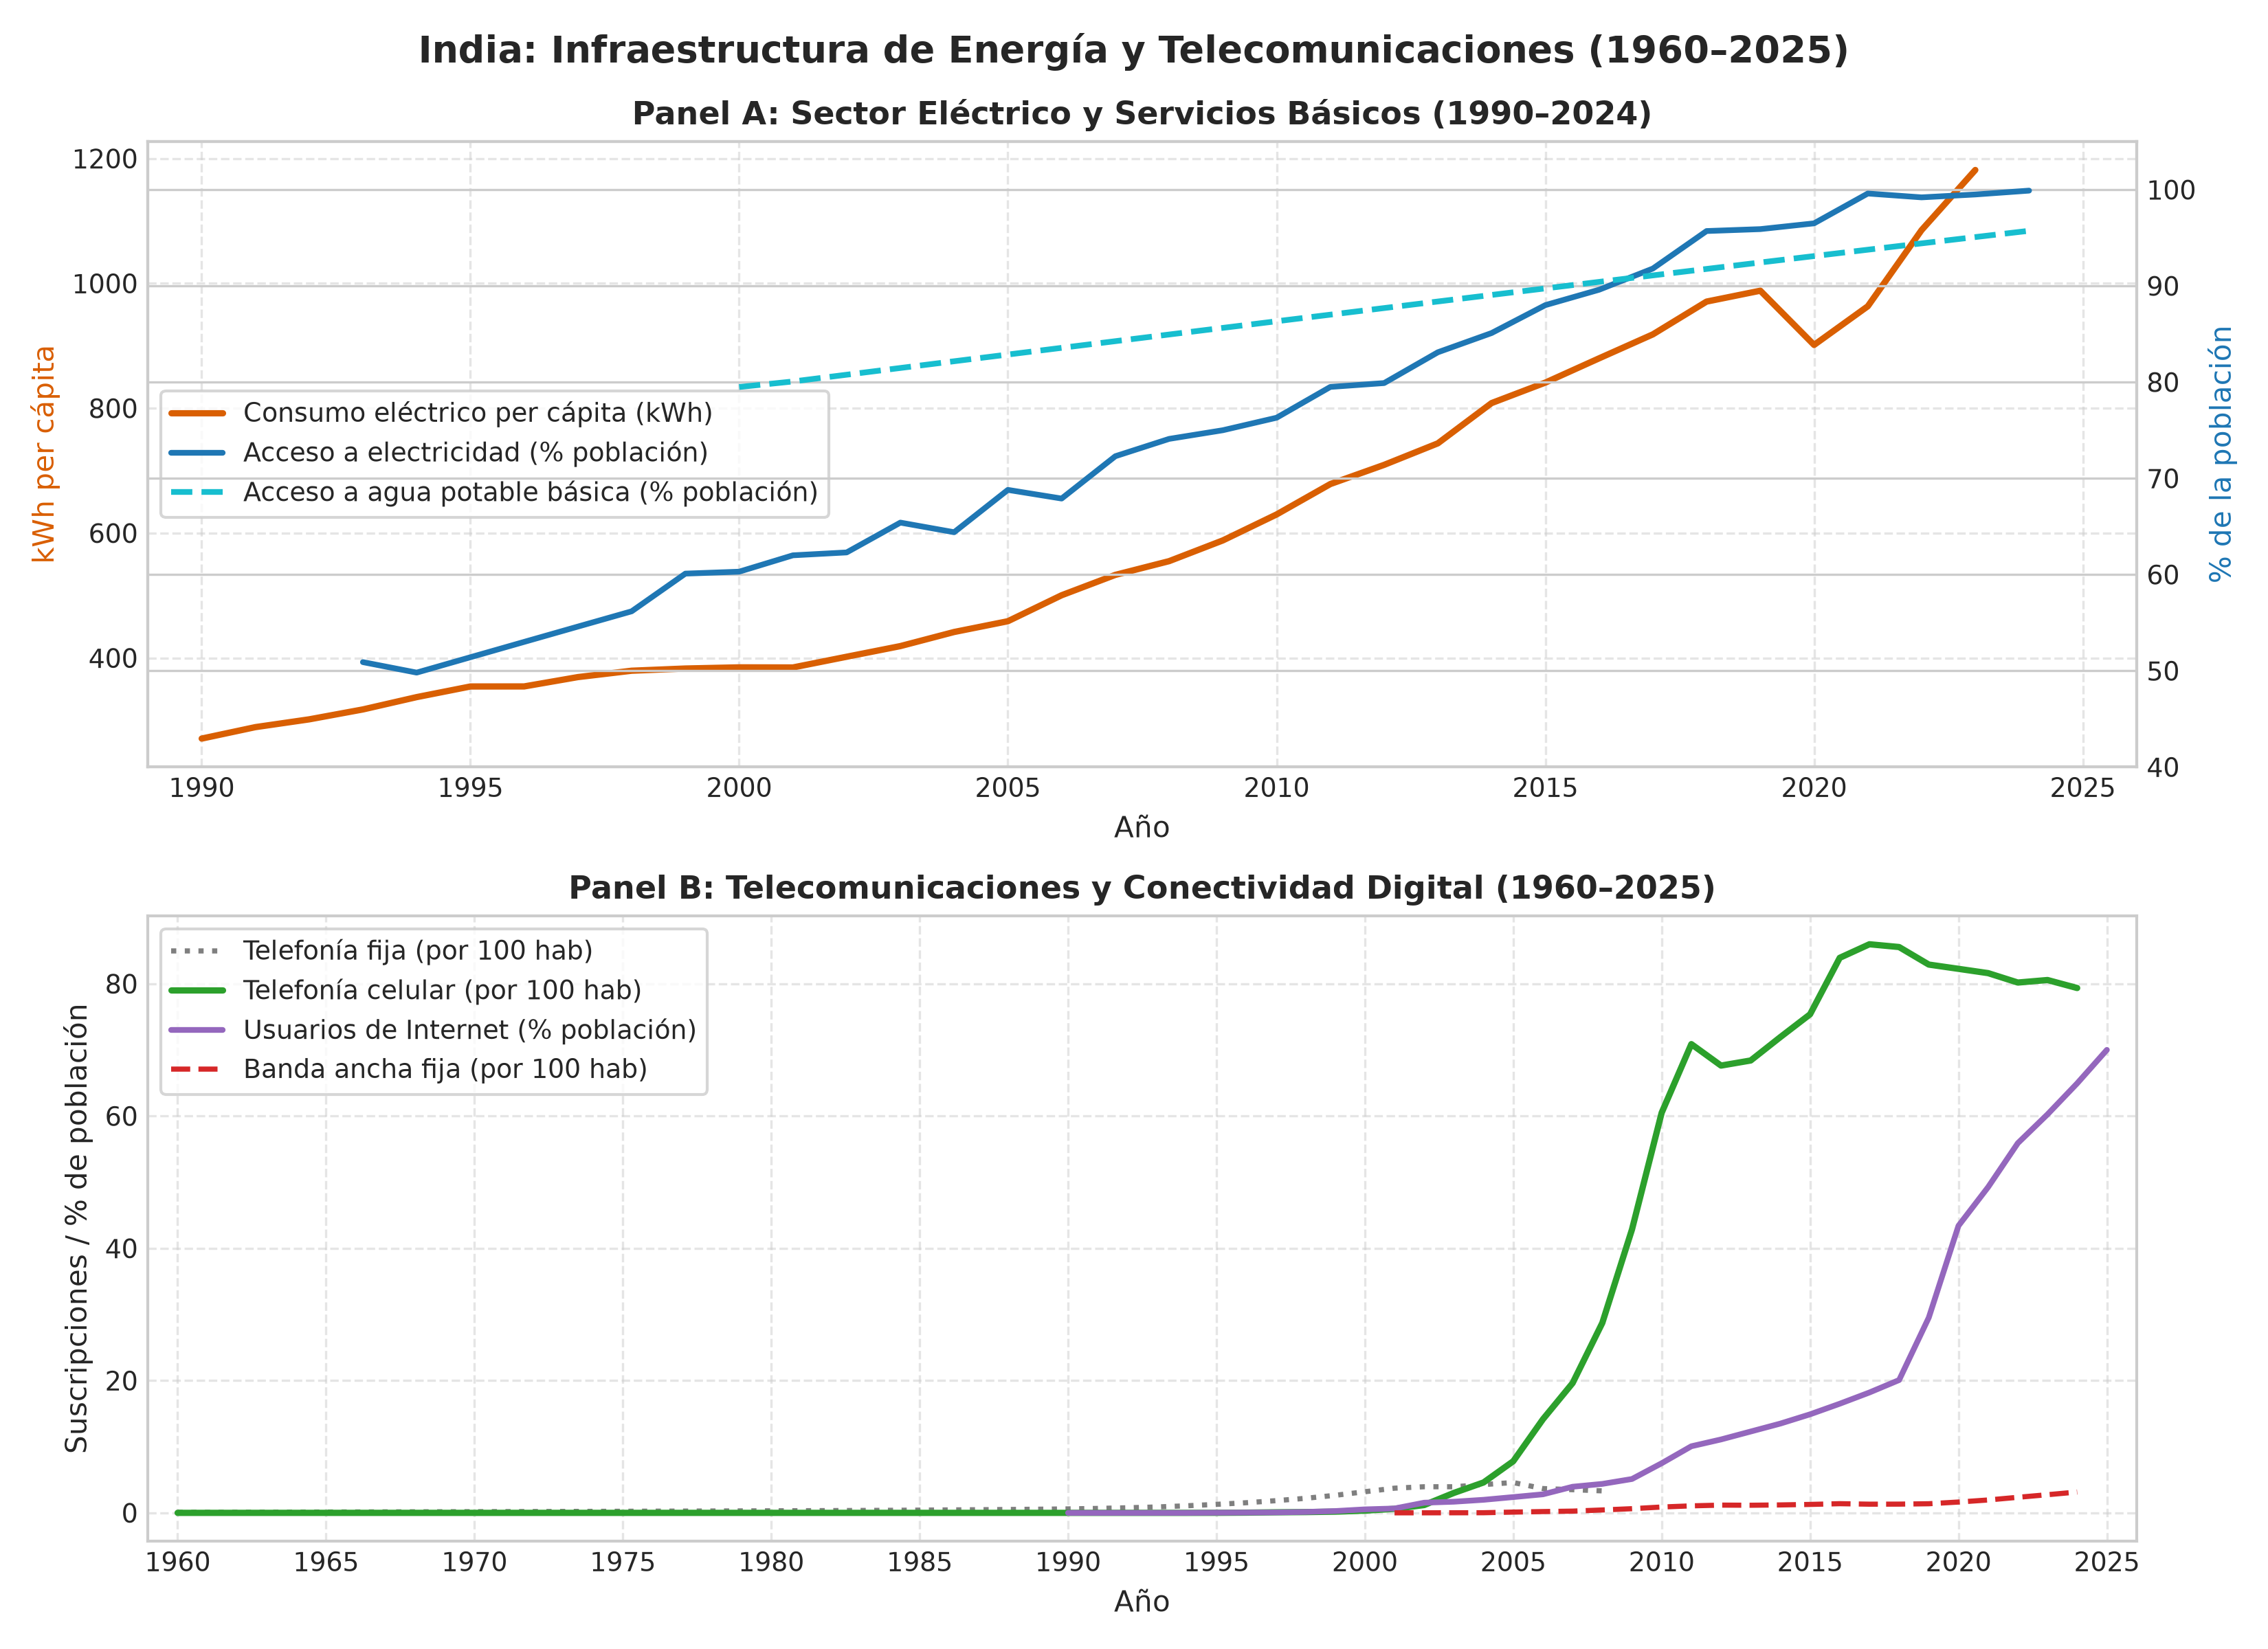
\includegraphics[width=0.98\textwidth]{output/figures/fig3_india_energia_telecomunicaciones_historico.png}
    \caption{\textbf{India: Infraestructura de Energía y Telecomunicaciones (1960--2025).} \\
    \textit{Panel A:} Consumo eléctrico per cápita (kWh) y acceso a electricidad y agua potable básica (\% población), 1990--2024. \textit{Panel B:} Transición de telefonía fija hacia telefonía celular, internet y banda ancha (suscripciones por 100 hab. / \% población), 1960--2025. Fuente: World Bank y EconStats.}
    \label{fig:energia_telecom}
\end{figure}

\noindent \textbf{Descripción breve:} La electrificación pasó de cubrir el 50\% de la población en 1993 a prácticamente el 100\% hacia 2020, cuadruplicando el consumo eléctrico per cápita. En telecomunicaciones, India protagonizó un salto directo (\textit{leapfrogging}) a la telefonía móvil e internet móvil, eludiendo la restricción histórica de la red alámbrica fija.

\vspace{1em}
\subsection{Zoom al Período del Big Push (2000--2015)}

La Figura~\ref{fig:zoom_bp} enfoca la ventana de aceleración más nítida para contrastar la hipótesis de coordinación simultánea.

\begin{figure}[H]
    \centering
    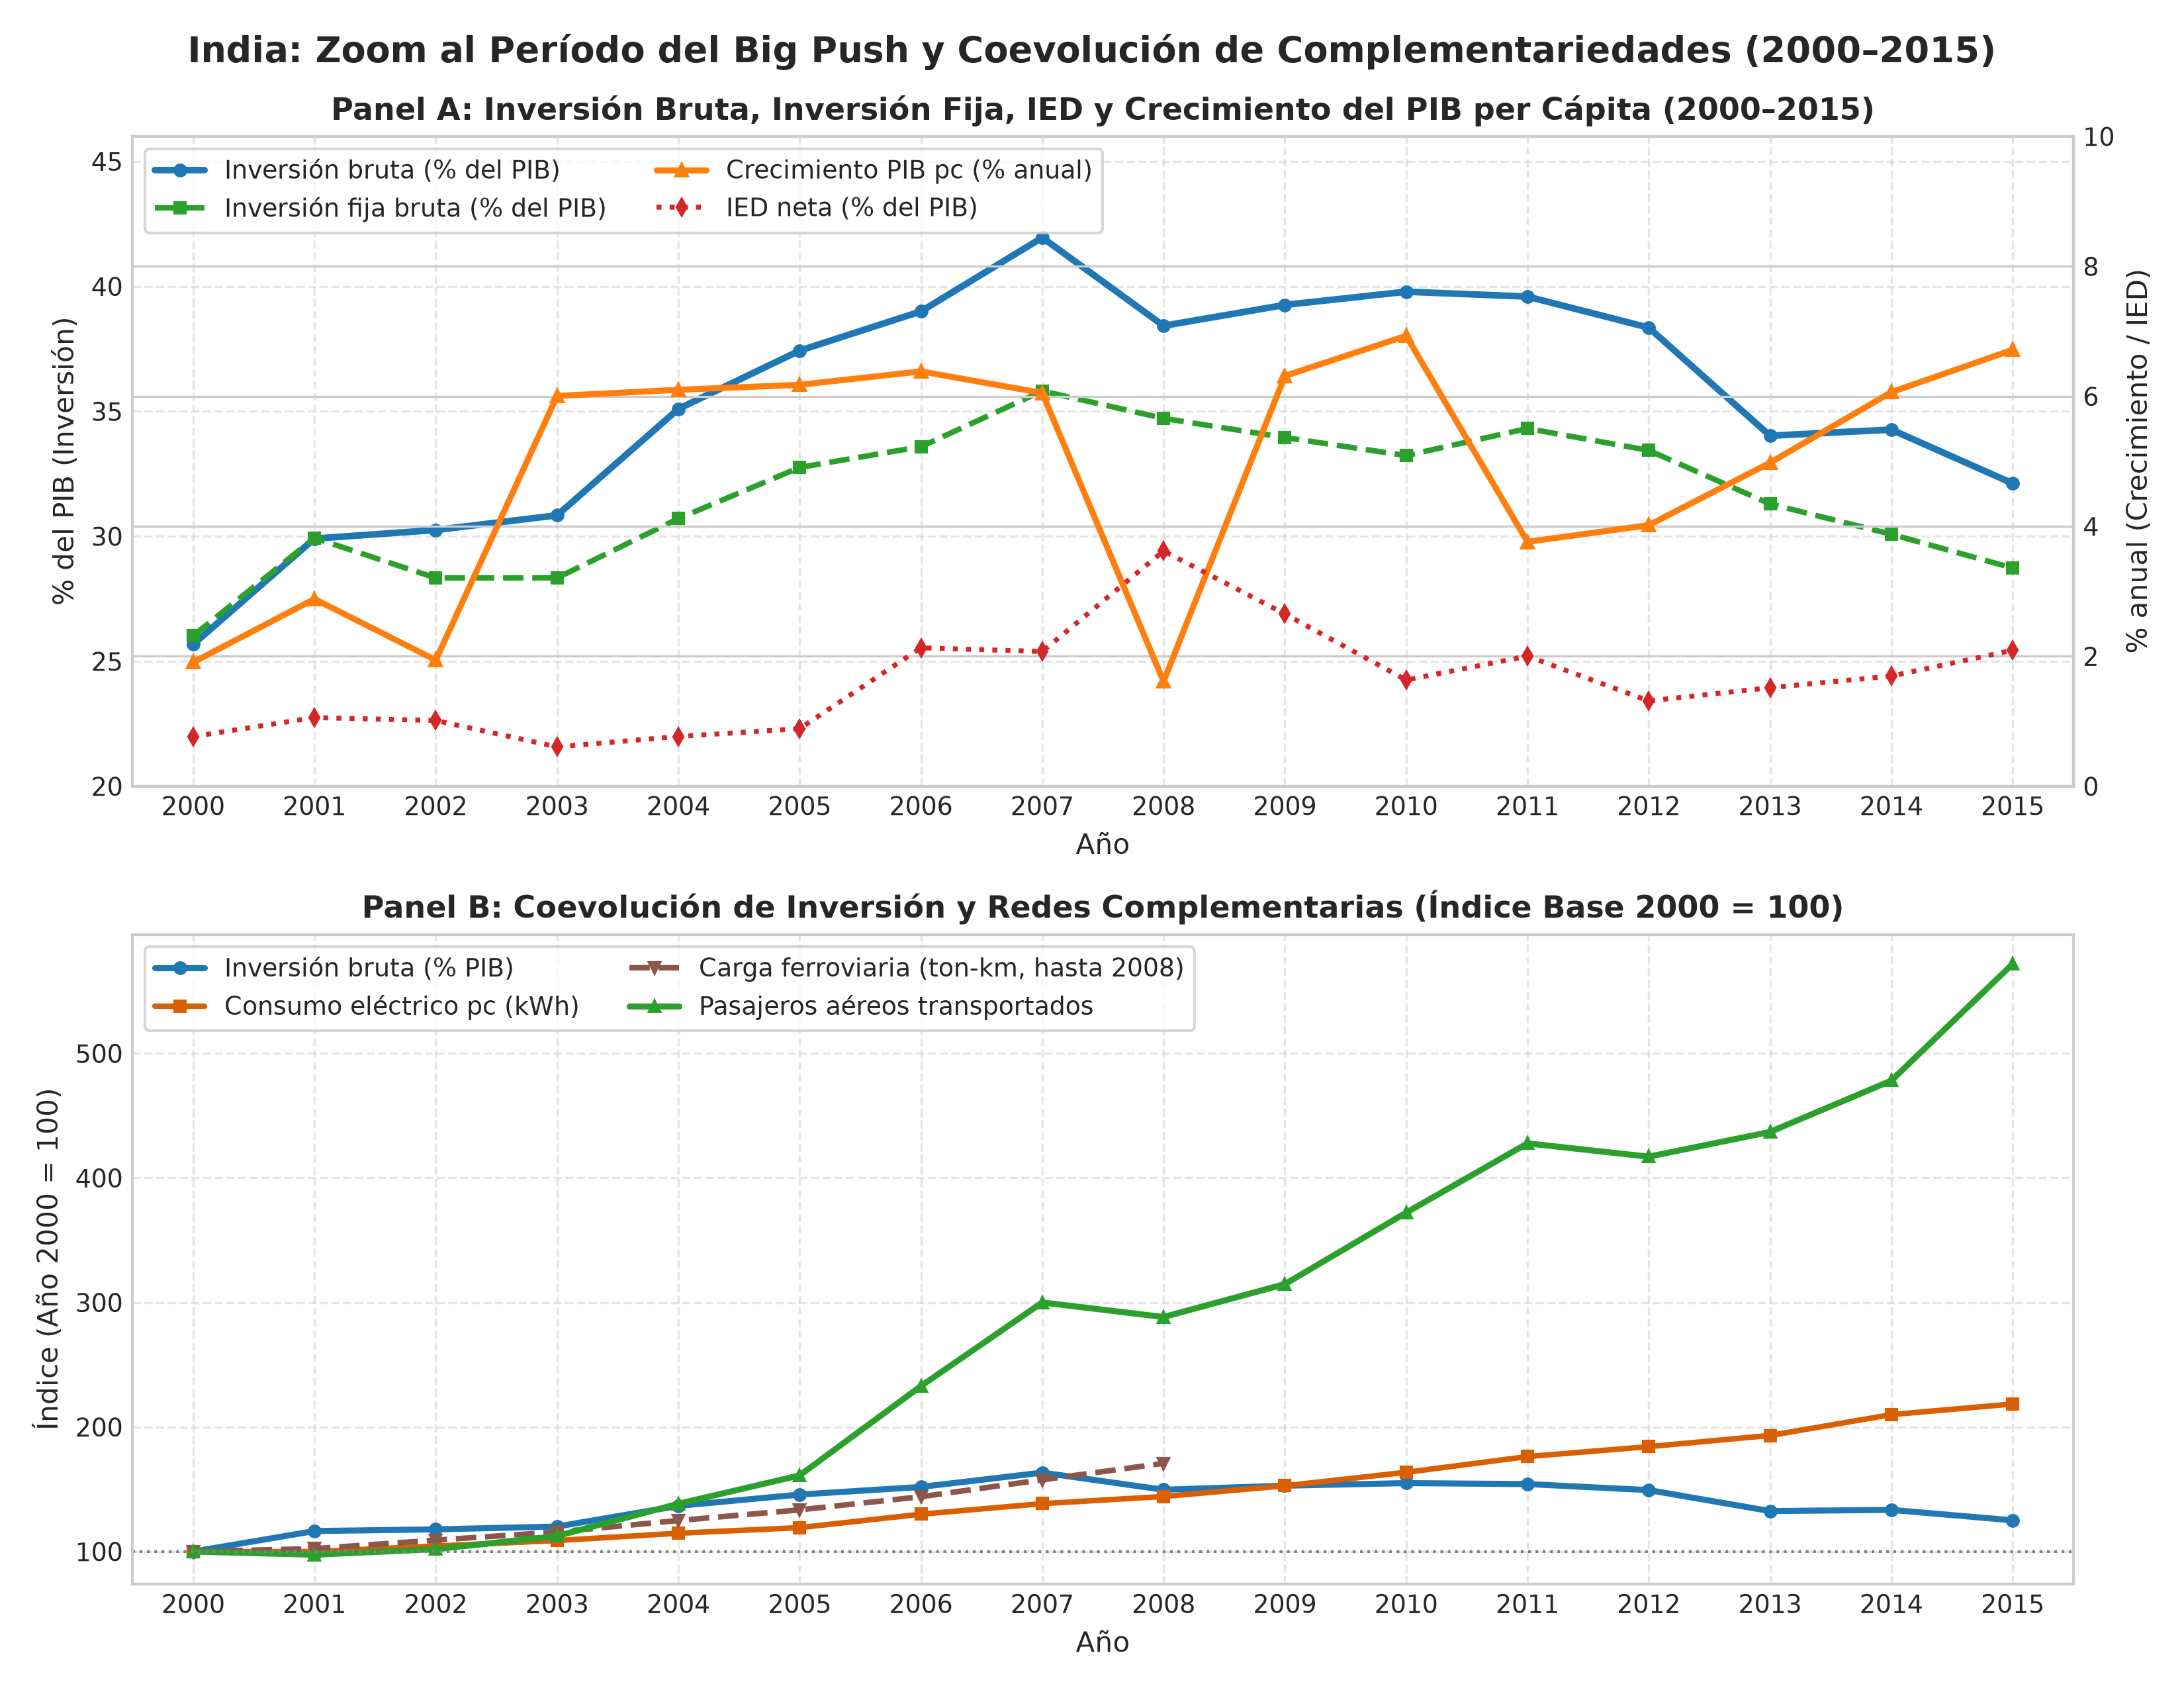
\includegraphics[width=0.98\textwidth]{output/figures/fig4_india_big_push_zoom_2000_2015.png}
    \caption{\textbf{India: Período del Big Push y Coevolución de Complementariedades (2000--2015).} \\
    \textit{Panel A:} Dinámica anual de inversión bruta, fija, IED y crecimiento del PIB per cápita. \textit{Panel B:} Coevolución simultánea de redes complementarias en series indexadas (Año 2000 = 100). Fuente: Elaboración propia en base a WDI y EconStats.}
    \label{fig:zoom_bp}
\end{figure}

\noindent \textbf{Descripción breve:} Entre 2003 y 2011 se cumplen los tres requisitos del \textit{Big Push}: aceleración del PIB pc ($>6.2\%$ promedio sostenido por 8 años), salto de la inversión al 42\% del PIB e ingreso récord de IED (3.6\% del PIB en 2008), coevolucionando con una expansión coordinada en carga de transporte, aviación y potencia eléctrica.

\newpage
\section{Parte 2: Crecimiento Equilibrado vs. Desequilibrado}

En este apartado se contrasta la teoría de crecimiento equilibrado de Nurkse (sincronismo sectorial para evitar cuellos de botella) con la teoría de crecimiento desequilibrado de Hirschman (sectores líderes con fuertes encadenamientos hacia atrás y adelante).

\subsection{Crecimiento Sectorial Histórico (1961--2025)}

La Figura~\ref{fig:sector_hist} abarca la trayectoria secular del valor agregado en Agricultura, Industria y Servicios junto con el PIB per cápita.

\begin{figure}[H]
    \centering
    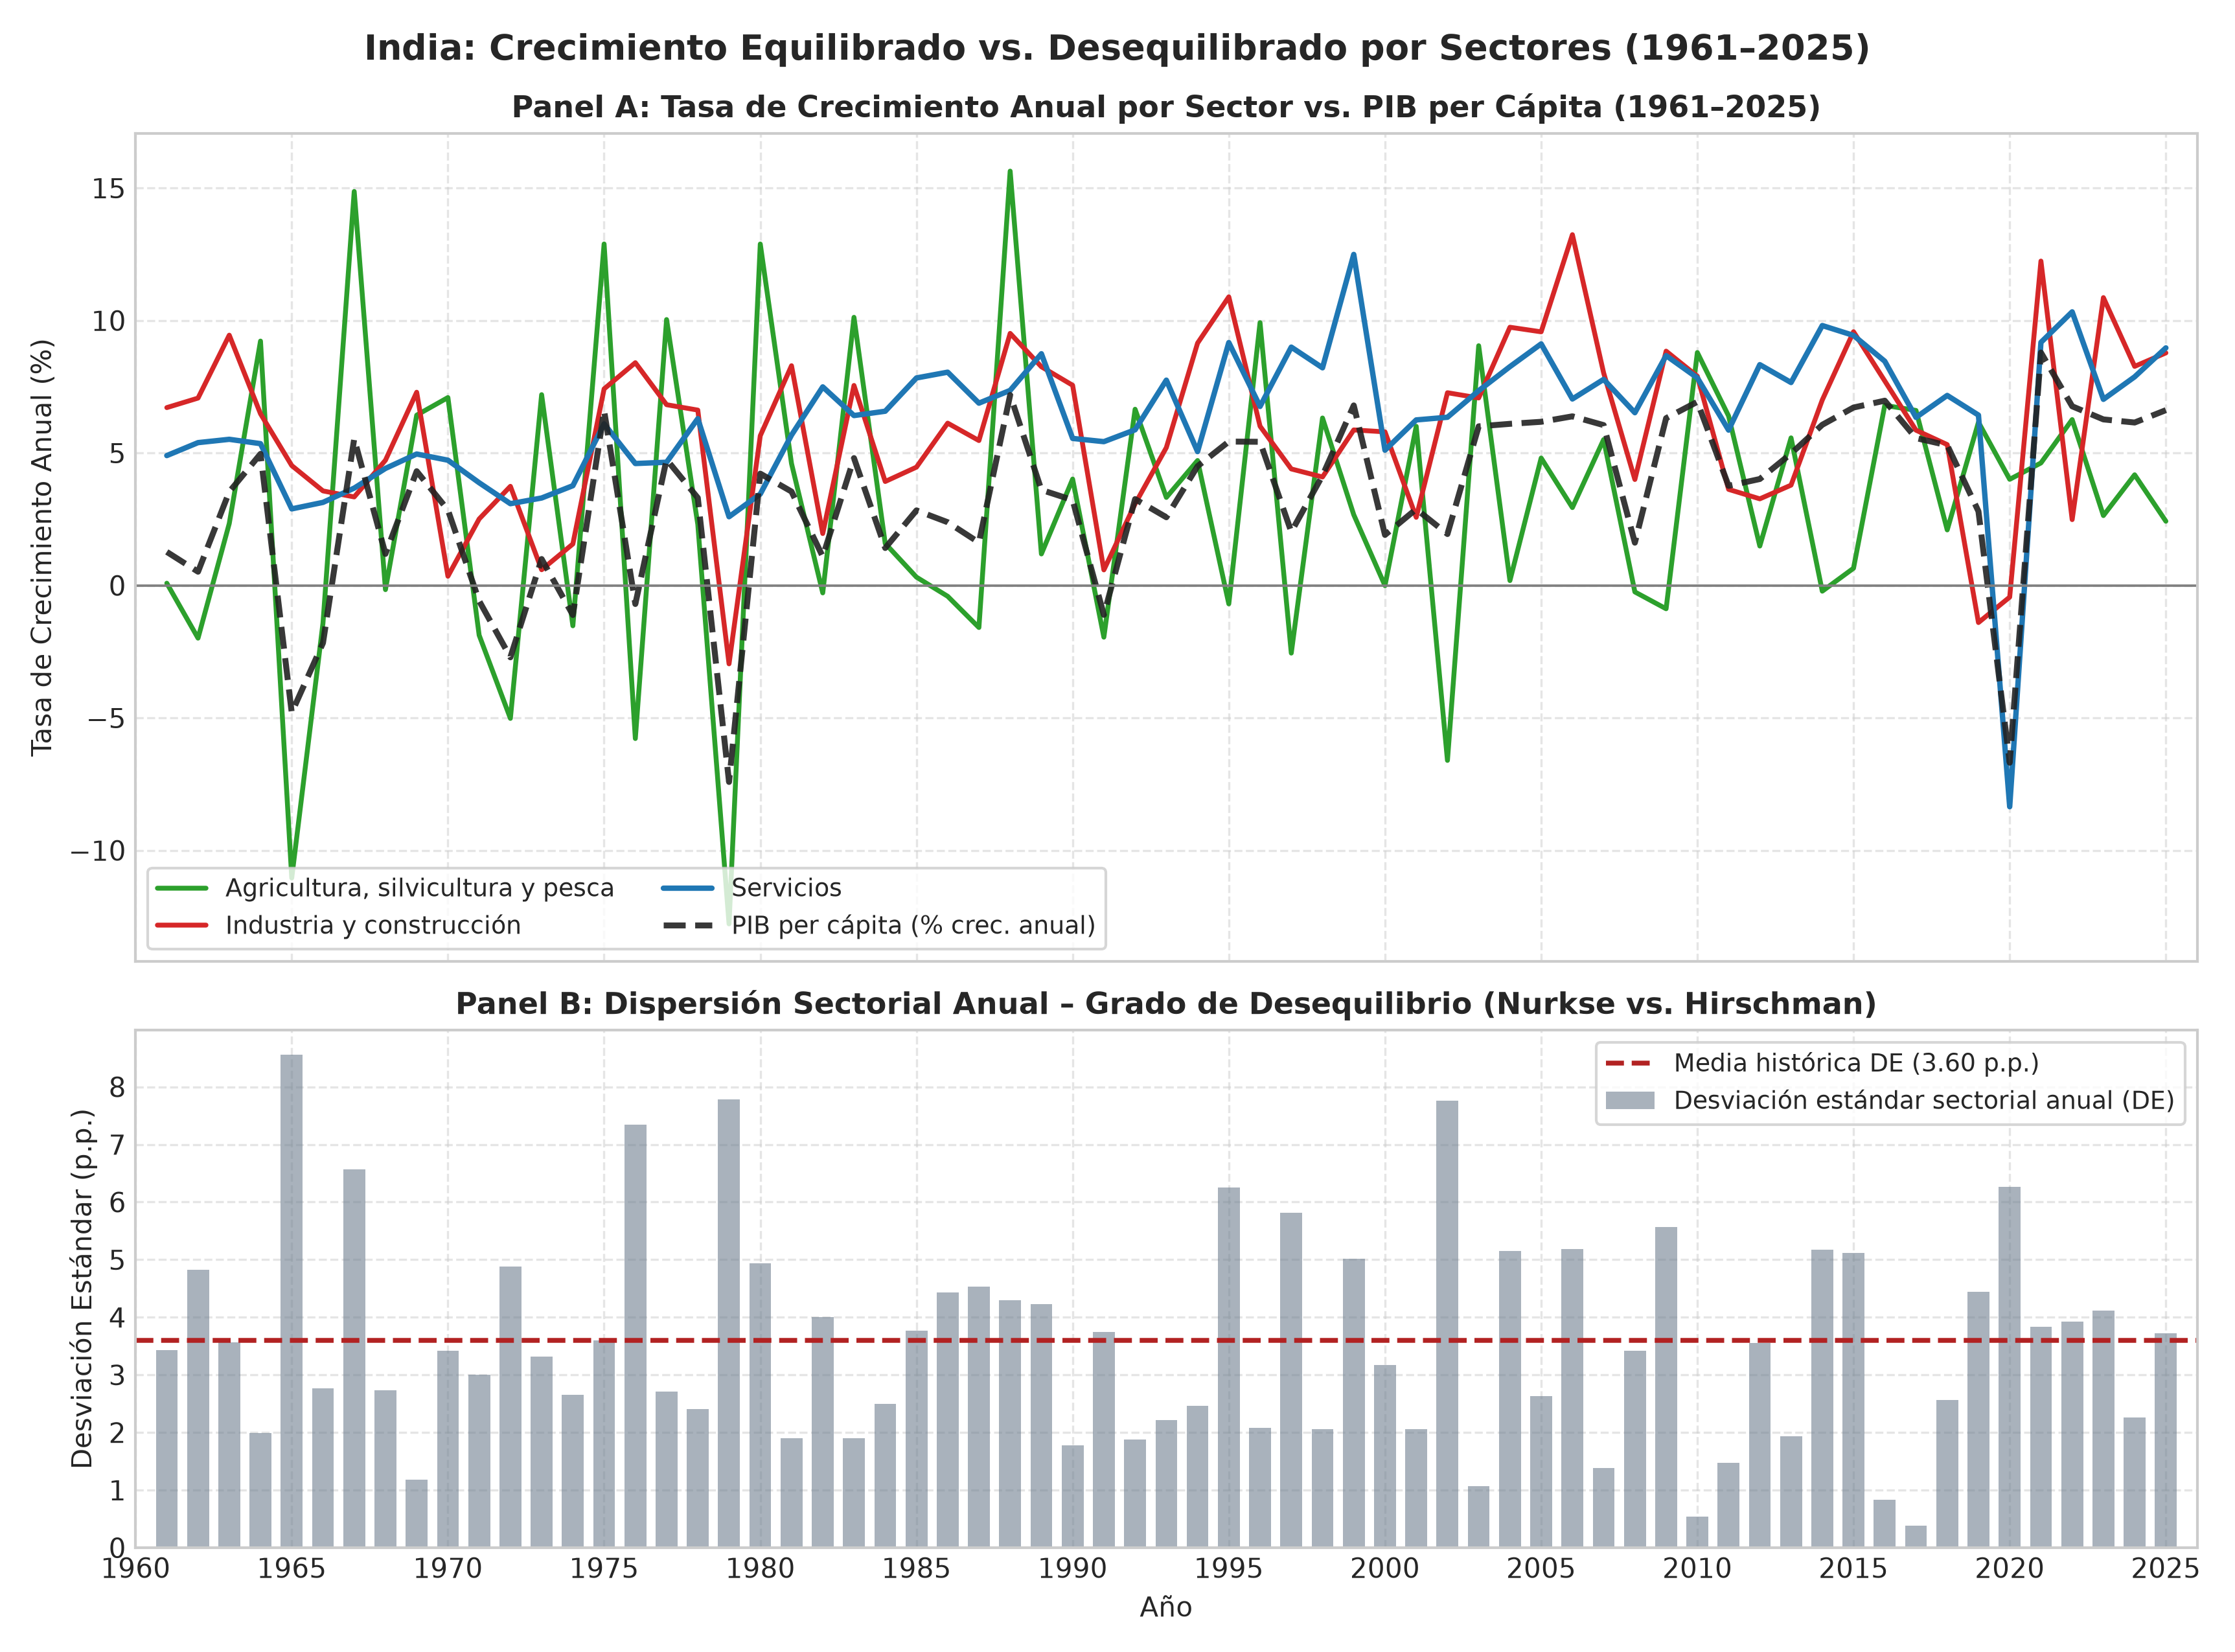
\includegraphics[width=0.98\textwidth]{output/figures/fig5_india_crecimiento_sectorial_historico.png}
    \caption{\textbf{India: Crecimiento Sectorial y Desequilibrio Transversal (1961--2025).} \\
    \textit{Panel A:} Crecimiento anual del valor agregado por sector frente al promedio del PIB per cápita. \textit{Panel B:} Desviación estándar transversal anual ($DE_t$) entre los tres sectores y media histórica de largo plazo (3.60 p.p.). Fuente: World Bank (WDI).}
    \label{fig:sector_hist}
\end{figure}

\noindent \textbf{Descripción breve:} Muestra la elevada volatilidad agrícola previa a 1990 y cómo, tras las reformas, los sectores de Servicios e Industria despegan con tasas sistemáticamente superiores al promedio de la economía.

\vspace{1em}
\subsection{Crecimiento Sectorial y Desequilibrio desde 1990}

La Figura~\ref{fig:sector_post90} presenta el ejercicio requerido por la consigna del práctico para el período 1990--2025.

\begin{figure}[H]
    \centering
    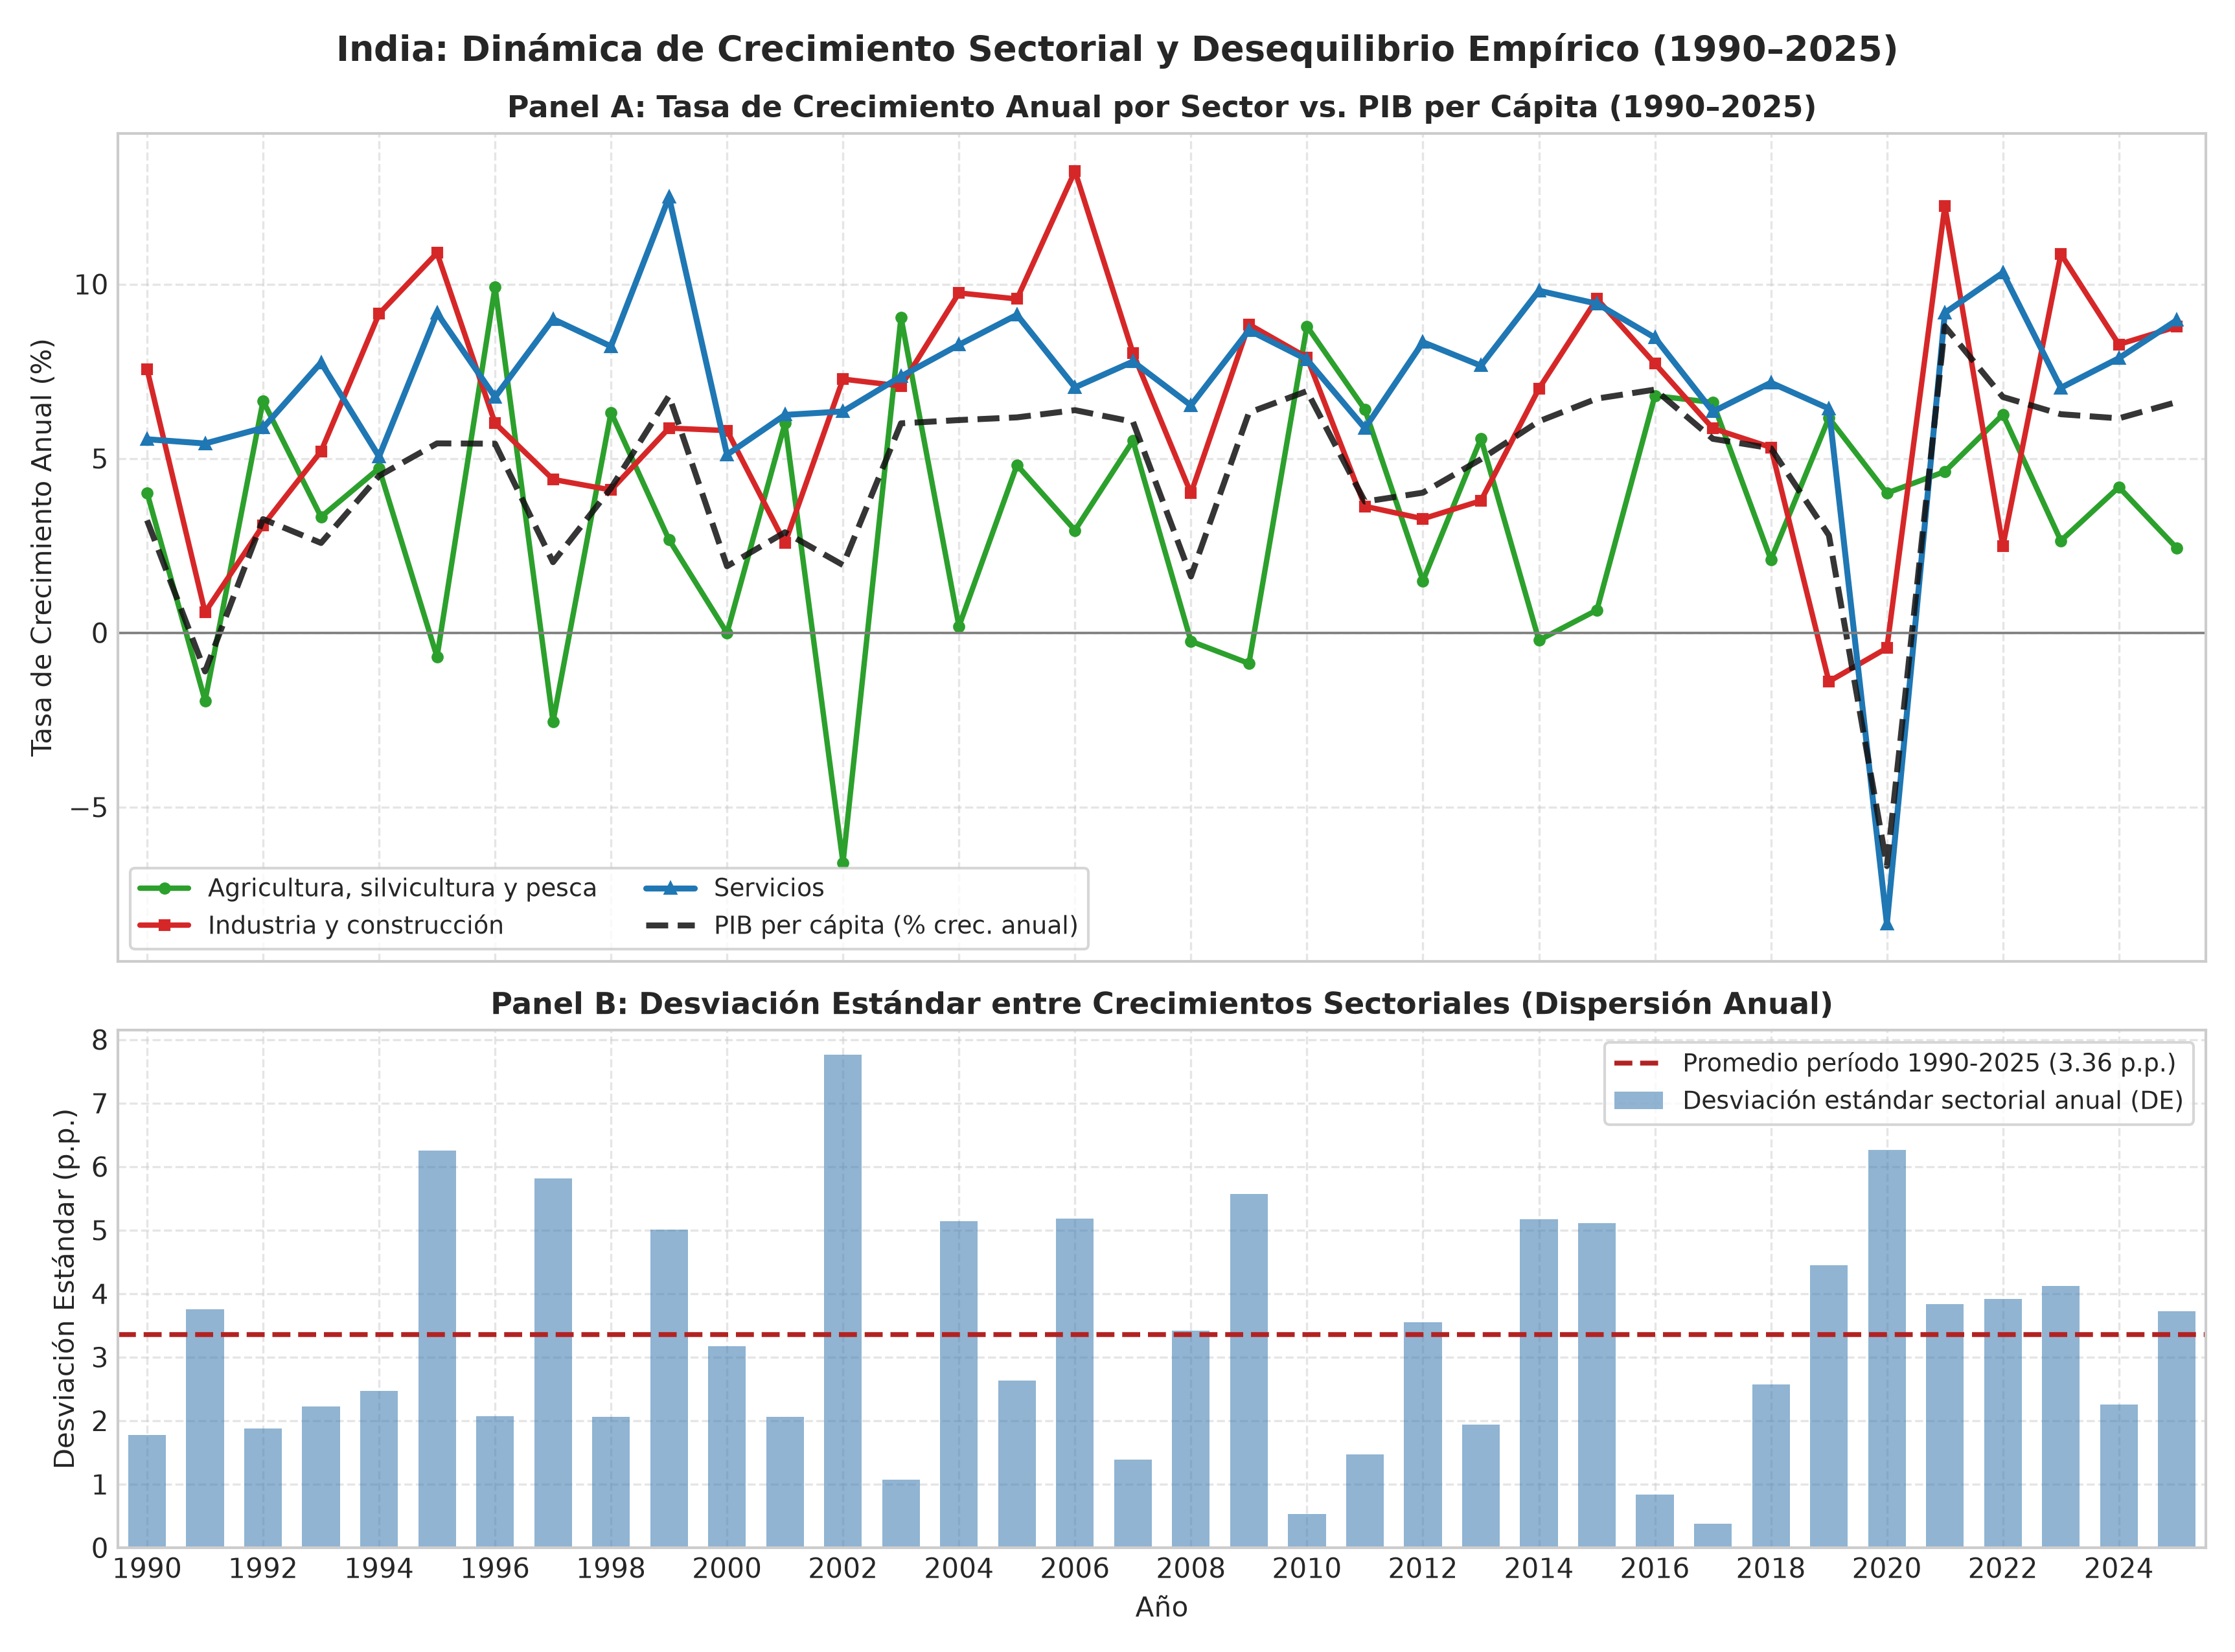
\includegraphics[width=0.98\textwidth]{output/figures/fig6_india_crecimiento_sectorial_desde_1990.png}
    \caption{\textbf{India: Dinámica de Crecimiento Sectorial y Desequilibrio Empírico (1990--2025).} \\
    \textit{Panel A:} Crecimiento anual por sector vs. PIB pc. \textit{Panel B:} Desviación estándar anual ($DE_t$) y promedio del período (3.36 p.p.). Mayor $DE_t$ indica desequilibrio (Hirschman); menor $DE_t$ indica sincronismo (Nurkse). Fuente: World Bank (WDI).}
    \label{fig:sector_post90}
\end{figure}

\noindent \textbf{Descripción breve:} Servicios actúa como sector líder permanente ($7$--$10\%$ anual), complementado por Industria en los picos de inversión. La dispersión sectorial ($DE_t$) alcanza picos de desequilibrio tipo Hirschman en 1995, 2002 ($7.76$ p.p.) y 2020, mientras que períodos como 2003, 2007, 2010 y 2016--2017 exhiben convergencia y crecimiento relativamente balanceado tipo Nurkse.

\end{document}
